\chapter{Illustration of Gesture Inference Results}
\label{Appendix3}

\section{Comparison between Ground Truth Gestures and Predicted Gestures}

\begin{center}
\centering
\href{https://youtu.be/22lNm2tvmrk}{% Replace with your YouTube URL
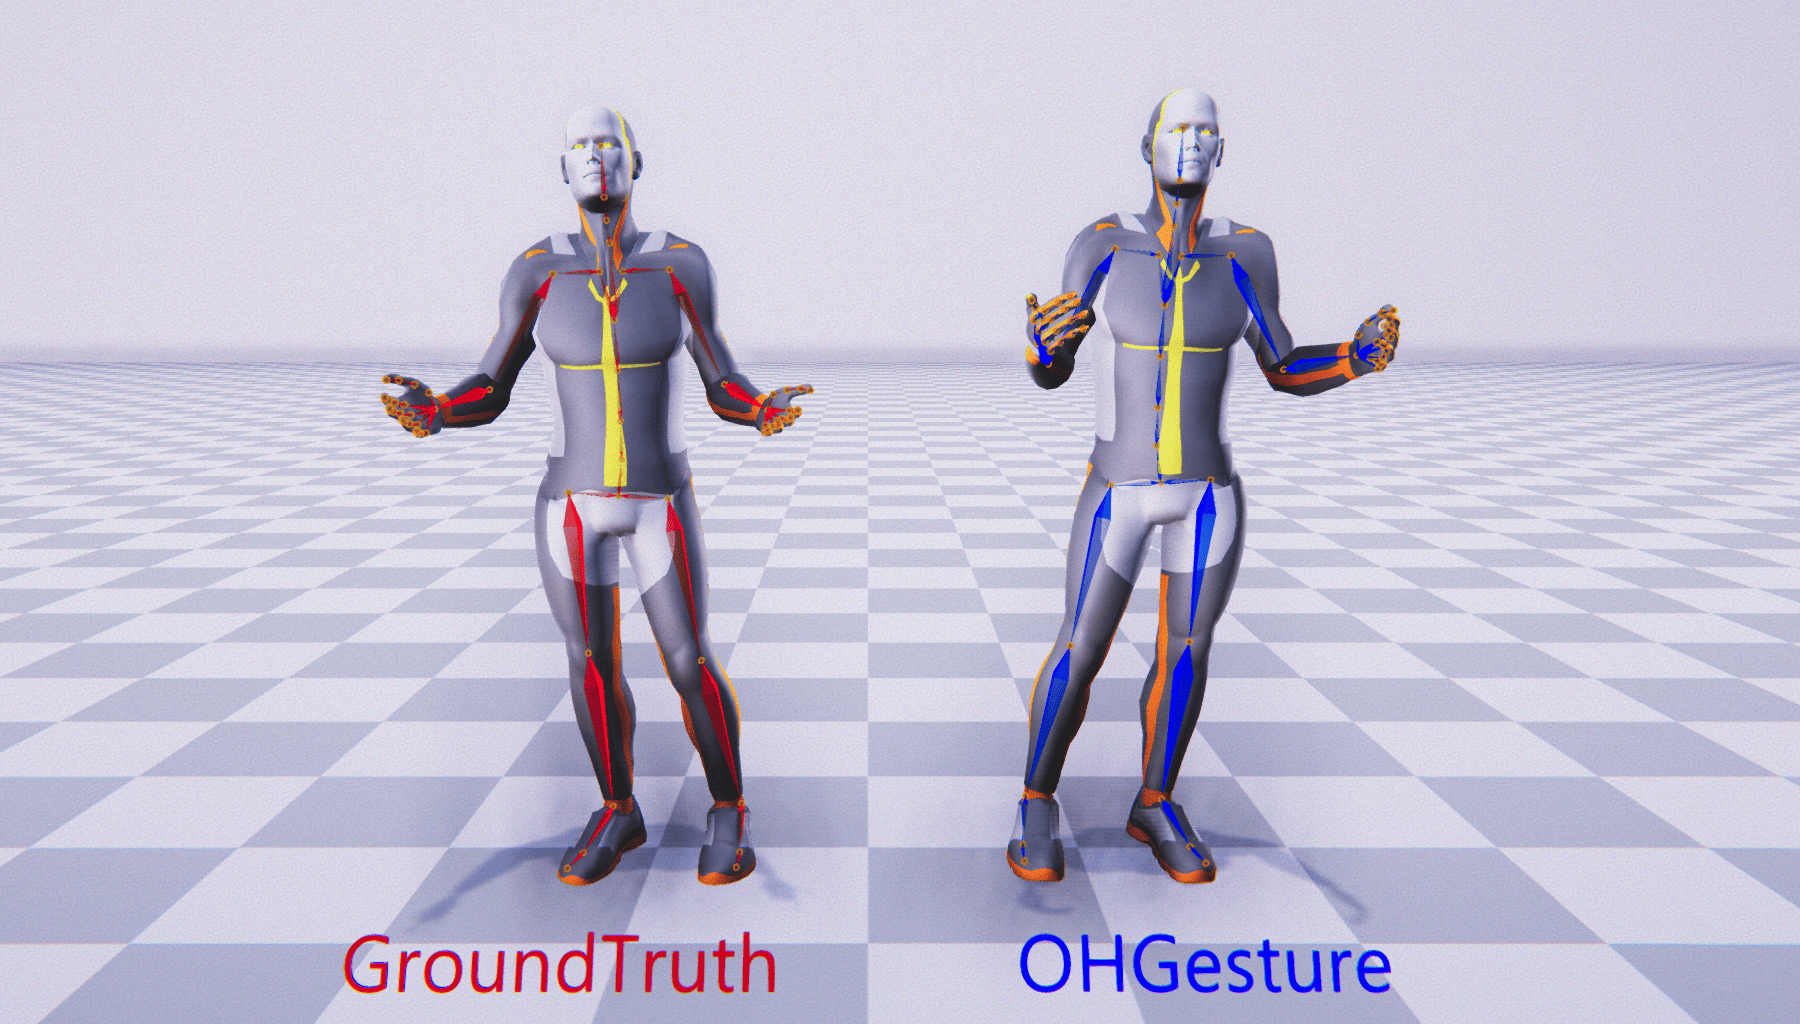
\includegraphics[width=\textwidth]{GroundTruthCompare}}
{\tiny Click the image to watch the video}
\end{center}

The results show both the ground truth gestures and the model's predicted gestures at frame $3821$, inferred from the speech sample $\texttt{003\_Neutral\_2\_x\_1\_0}$.

\section{Illustration of Different Emotions in Gestures}

{
	\begin{center}
		\centering
		\href{https://youtu.be/KUlBZXLtYJ4}{% Replace with your YouTube URL
			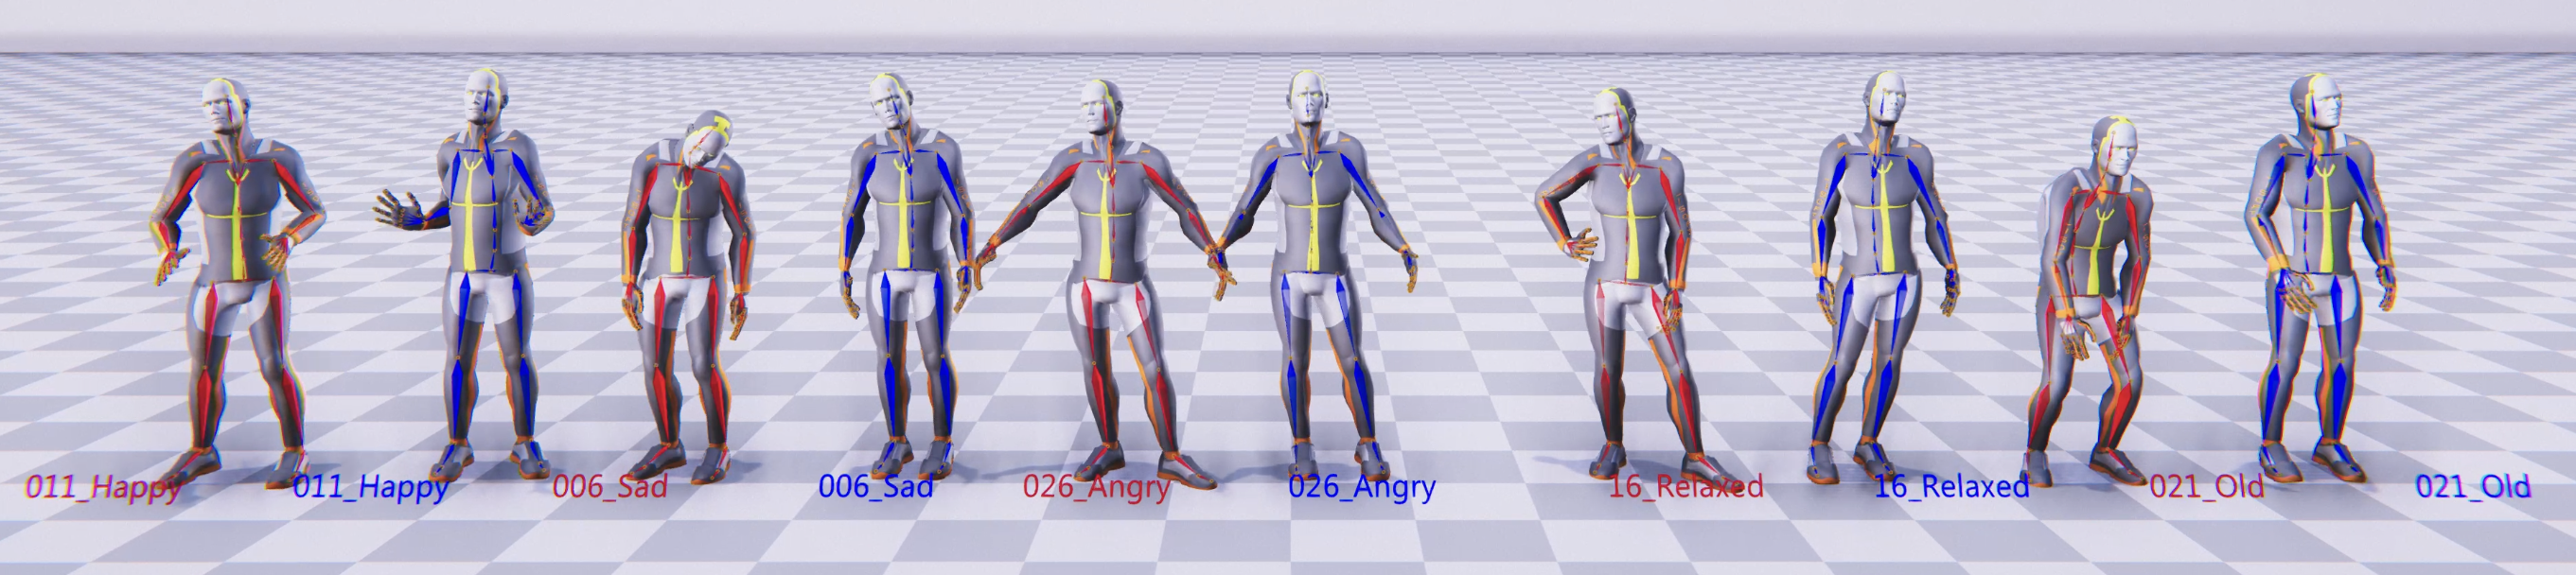
\includegraphics[width=\textwidth]{DifferenceEmotion}}
		
		{\tiny Click the image to watch the video}
	\end{center}
}

Generated or inferred results from the OHGesture model with different emotions. Red indicates the ground truth from the ZeroEGGS dataset, while blue shows the output generated by the OHGesture model.

{
	\begin{center}
		\centering
		\href{https://youtu.be/eZghfNGmZn8}{% Replace with your YouTube URL
			\includegraphics[width=\textwidth]{ListOfEmotion}}
		
		{\tiny Click the image to watch the video}
	\end{center}
}

\section{Illustration of Gesture Generation with Out-of-Training Speech}

{
	\begin{center}
		\centering
		\href{https://www.youtube.com/watch?v=B6nv1kQmi-Q}{% Replace with your YouTube URL
		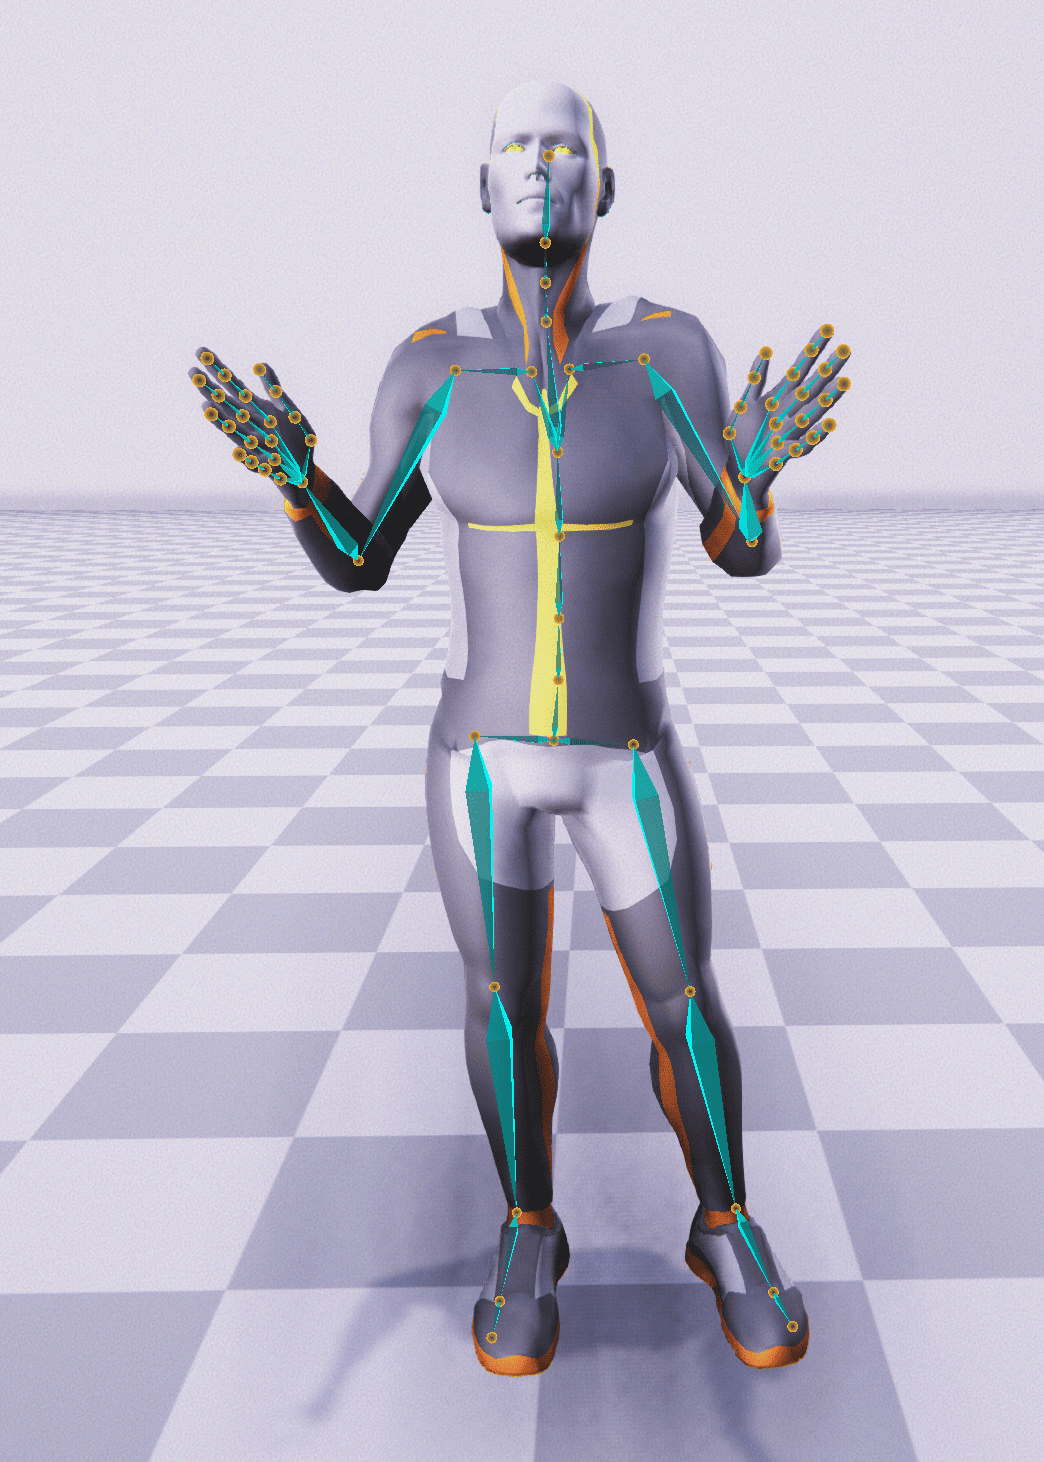
\includegraphics[width=0.4\textwidth]{StevenJob}}
		
		{\tiny Click the image to watch the video}
	\end{center}
}

Illustration of gesture generation corresponding to Steve Jobs’ speech.

{
	\begin{center}
		\centering
		\href{https://youtu.be/yLwXdm7UgPE}{% Replace with your YouTube URL
			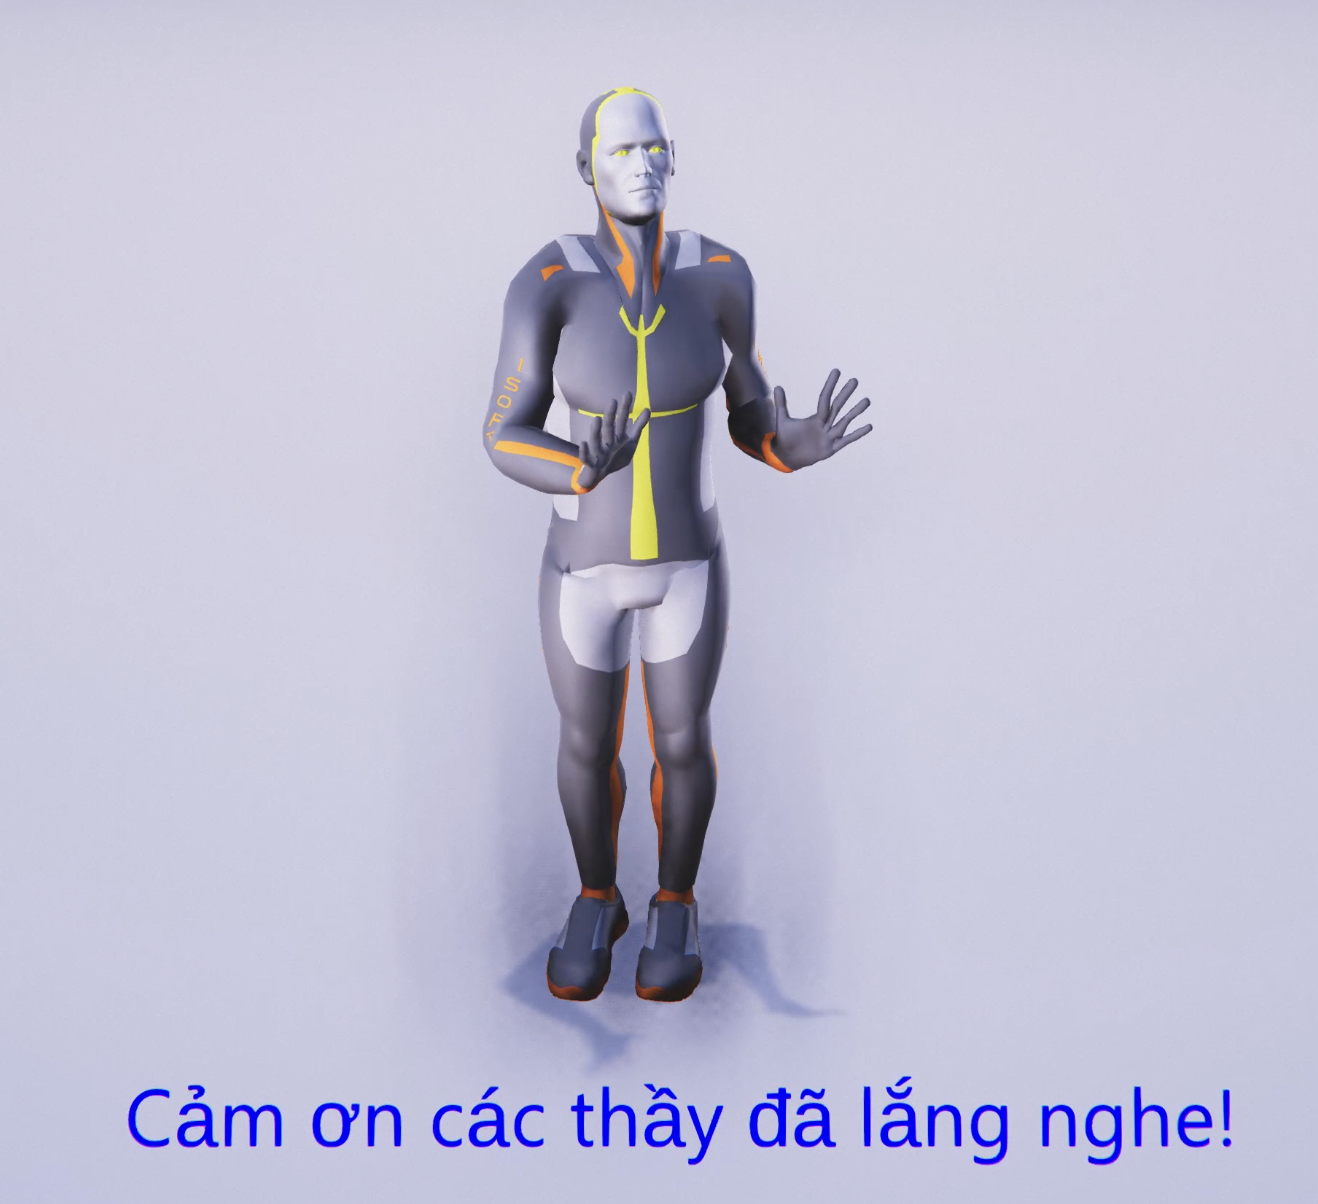
\includegraphics[width=0.6\textwidth]{OHGestureDemo}}
		
		{\tiny Click the image to watch the video}
	\end{center}
}

Illustration of gesture generation with synthesized speech from Microsoft Azure introducing the topic.

\section{Illustration of Character Motion}

\begin{center}
{
	\centering
	\href{https://www.youtube.com/watch?v=9IIIZP3EJLg}{% Replace with your YouTube URL
	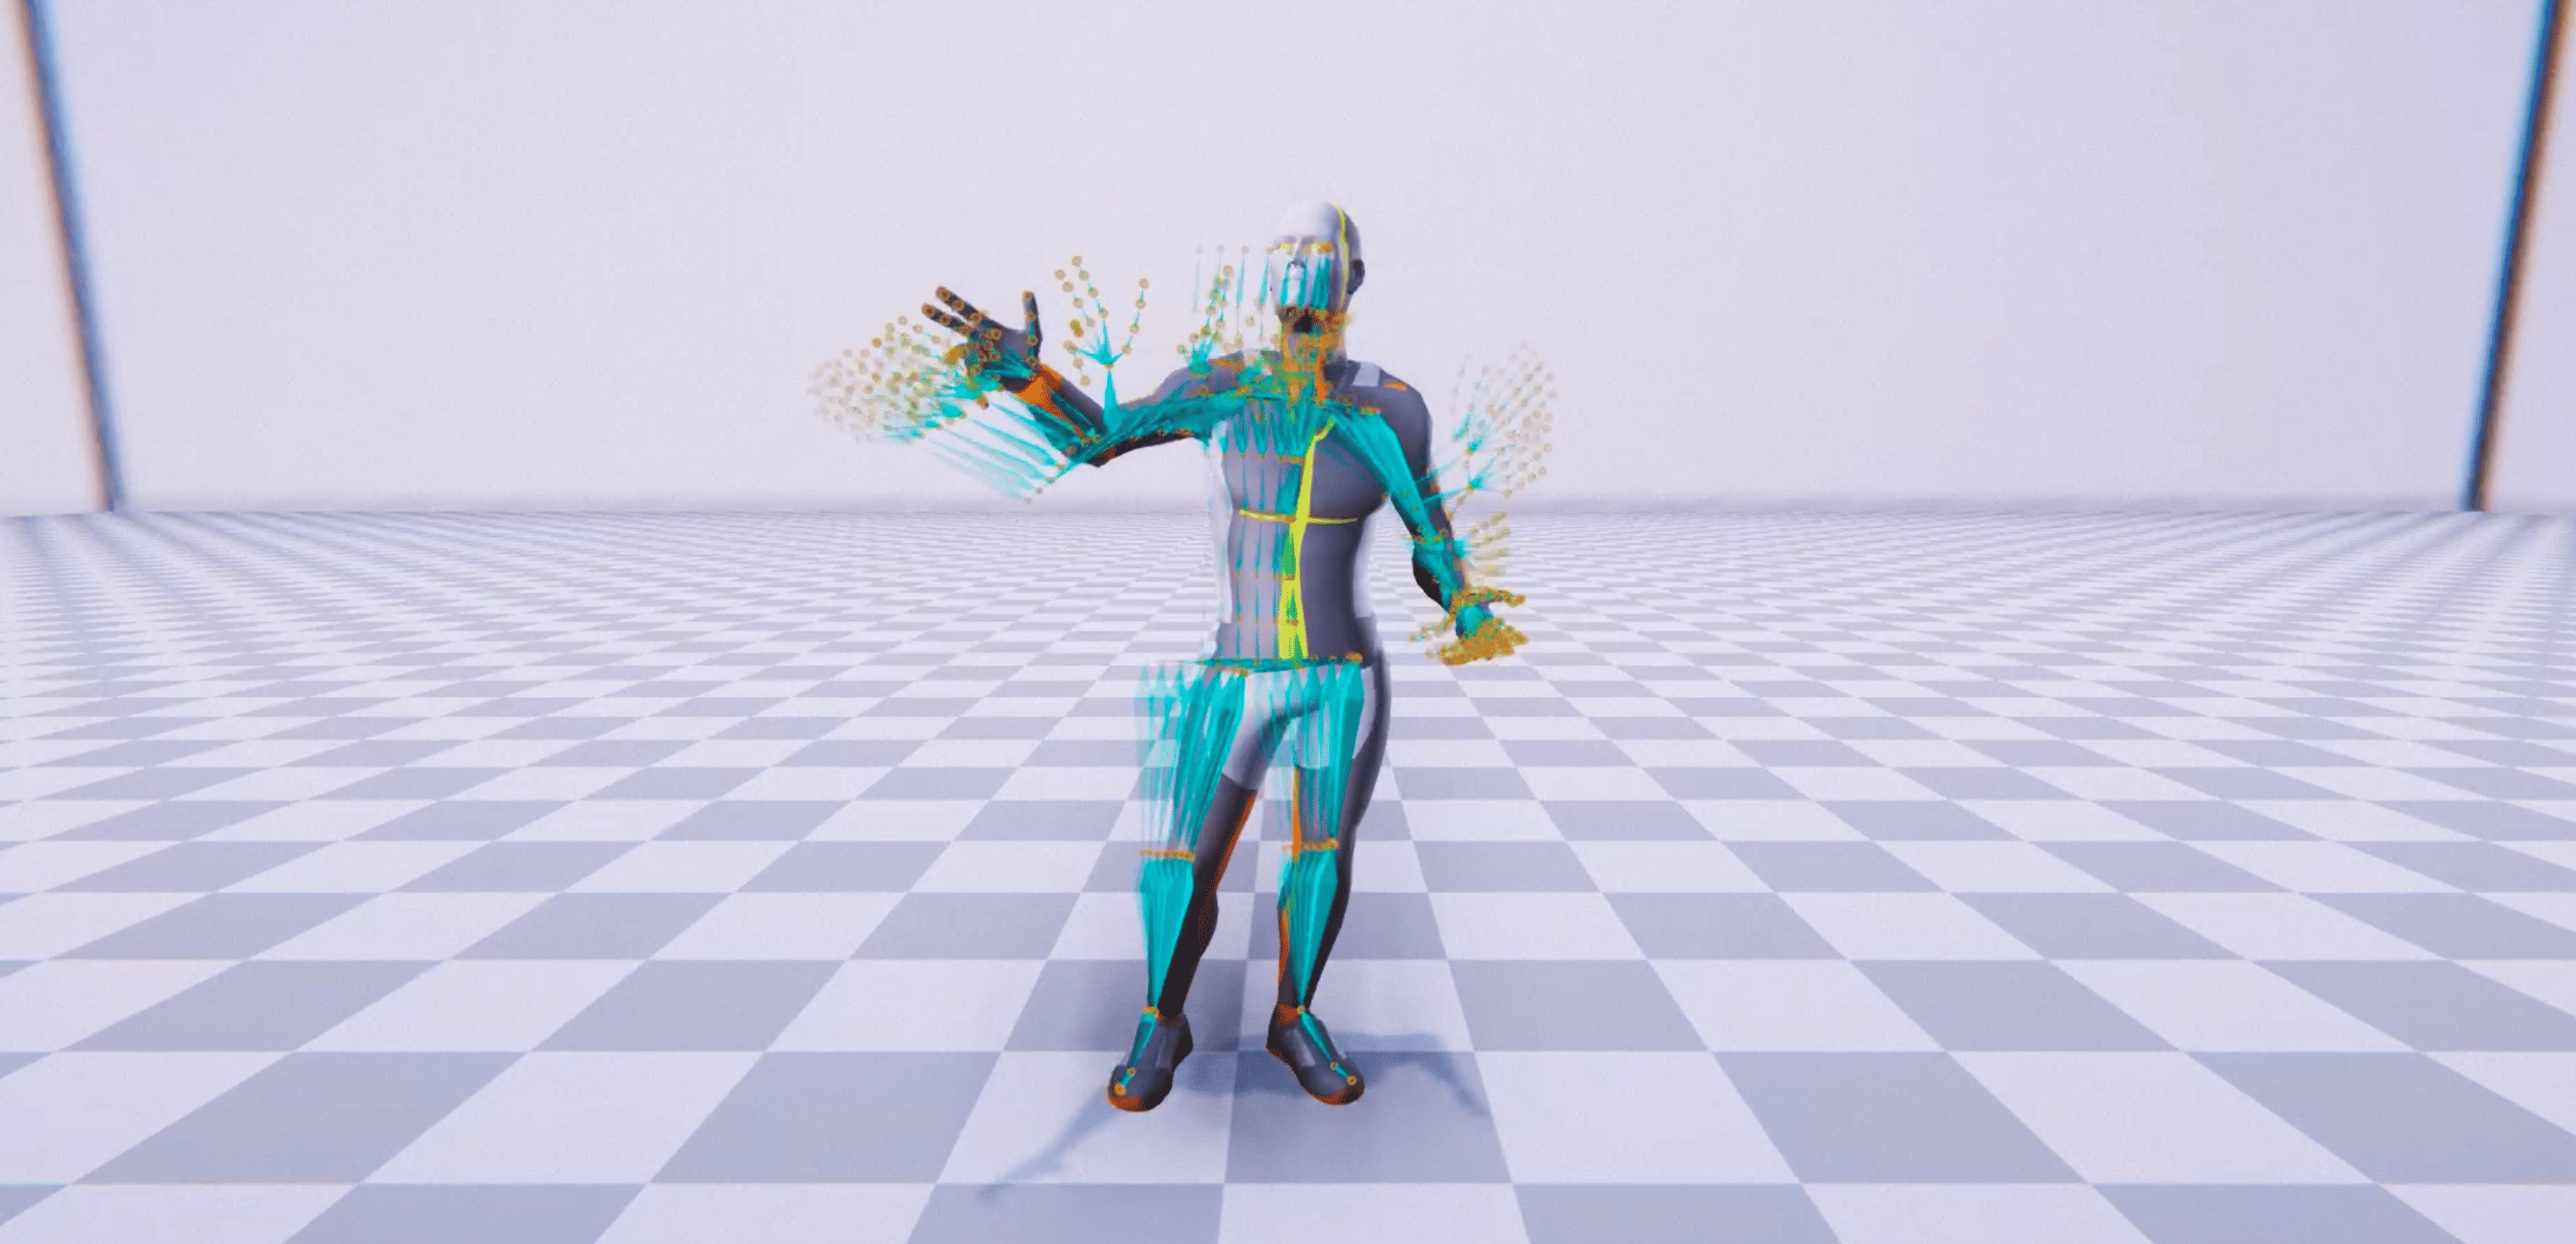
\includegraphics[width=0.8\textwidth]{DemoMotionGesture}}
	
	{\tiny Click the image to watch the video}
}
\end{center}
Illustration of gestures extracted from 6 frames before and 6 frames after the target gesture.
